\section*{Introduction}

PBImgAnalysis is a C library providing structures and functions to perform various data analysis on images.\\ 

It implements the following algorithms:
\begin{itemize}
\item K-means clustering on the RGBA space
\end{itemize}

It uses the \begin{ttfamily}PBErr\end{ttfamily}, \begin{ttfamily}PBDataAnalaysis\end{ttfamily}, \begin{ttfamily}GenBrush\end{ttfamily} libraries.\\

\section{Interface}

\begin{scriptsize}
\begin{ttfamily}
\verbatiminput{/home/bayashi/GitHub/PBImgAnalysis/pbimganalysis.h}
\end{ttfamily}
\end{scriptsize}

\section{Code}

\subsection{pbimganalysis.c}

\begin{scriptsize}
\begin{ttfamily}
\verbatiminput{/home/bayashi/GitHub/PBImgAnalysis/pbimganalysis.c}
\end{ttfamily}
\end{scriptsize}

\section{Makefile}

\begin{scriptsize}
\begin{ttfamily}
\verbatiminput{/home/bayashi/GitHub/PBImgAnalysis/Makefile}
\end{ttfamily}
\end{scriptsize}

\section{Unit tests}

\begin{scriptsize}
\begin{ttfamily}
\verbatiminput{/home/bayashi/GitHub/PBImgAnalysis/main.c}
\end{ttfamily}
\end{scriptsize}

\section{Unit tests output}

\begin{scriptsize}
\begin{ttfamily}
\verbatiminput{/home/bayashi/GitHub/PBImgAnalysis/unitTestRef.txt}
\end{ttfamily}
\end{scriptsize}

\subsection{K-Means clustering on RGBA space}

imgkmeanscluster01.tga:\\
\begin{center}
\begin{figure}[H]
\centering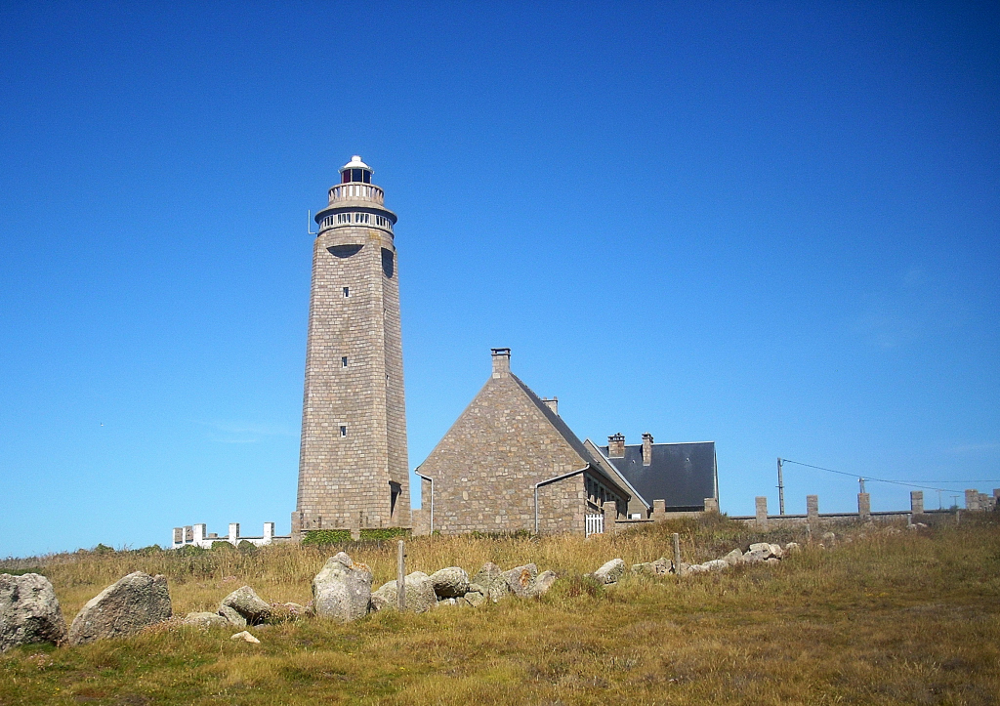
\includegraphics[width=6cm]{./imgkmeanscluster01.png}\\
\end{figure}
\end{center}

clustering for K equals 2 to 10:\\
\begin{center}
\begin{figure}[H]
\centering
\includegraphics[width=6cm]{./imgkmeanscluster01-02.png}
\centering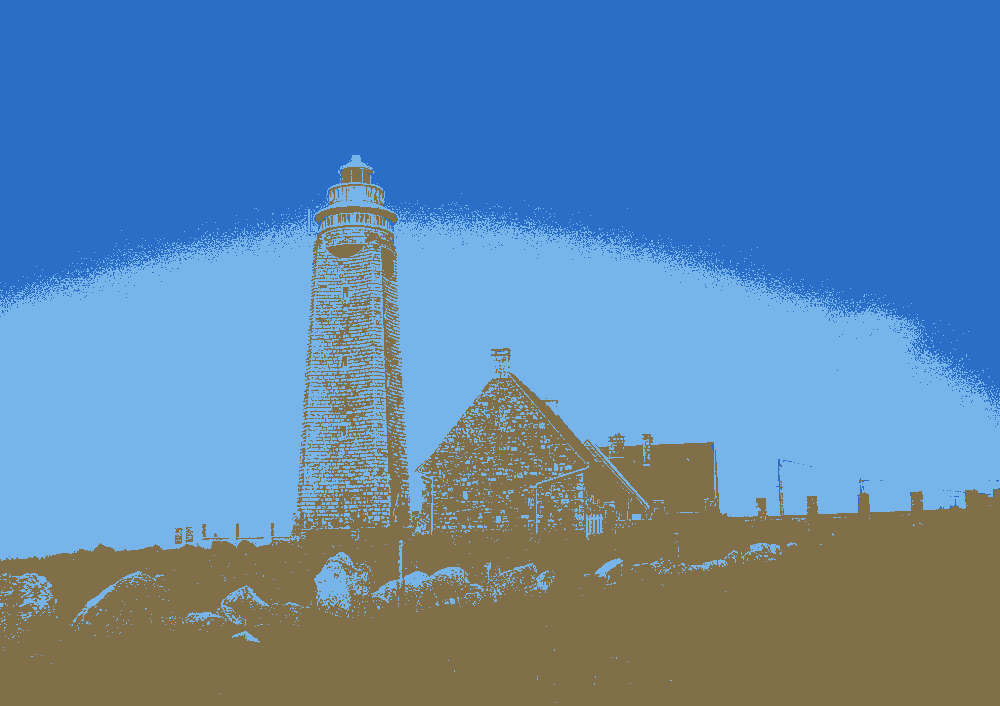
\includegraphics[width=6cm]{./imgkmeanscluster01-03.png}\\
\centering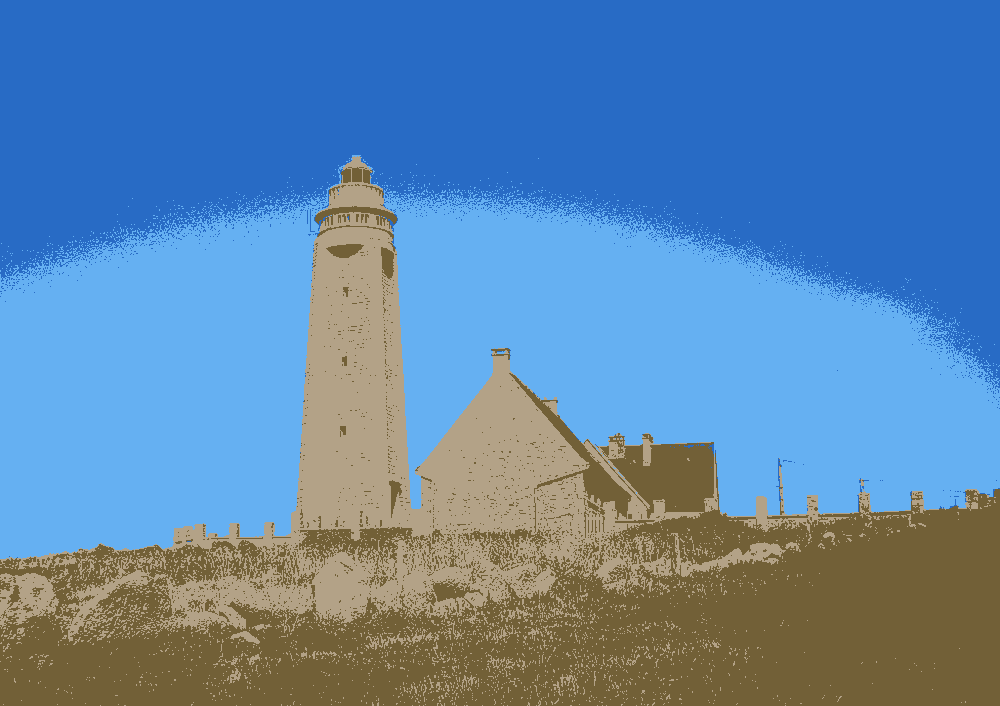
\includegraphics[width=6cm]{./imgkmeanscluster01-04.png}
\centering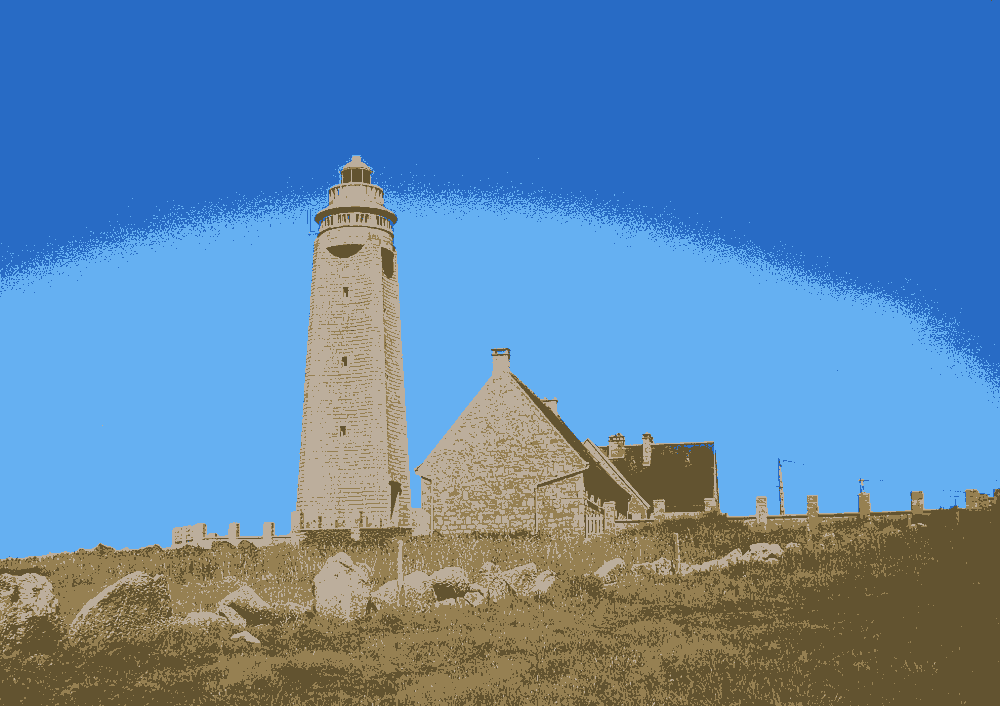
\includegraphics[width=6cm]{./imgkmeanscluster01-05.png}\\
\centering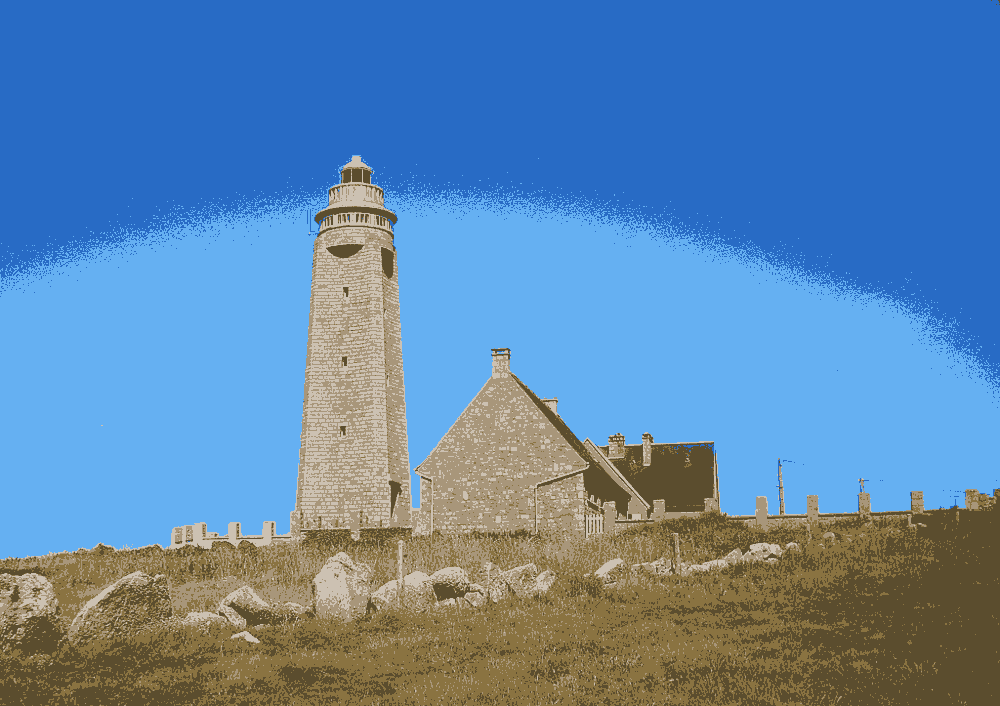
\includegraphics[width=6cm]{./imgkmeanscluster01-06.png}
\centering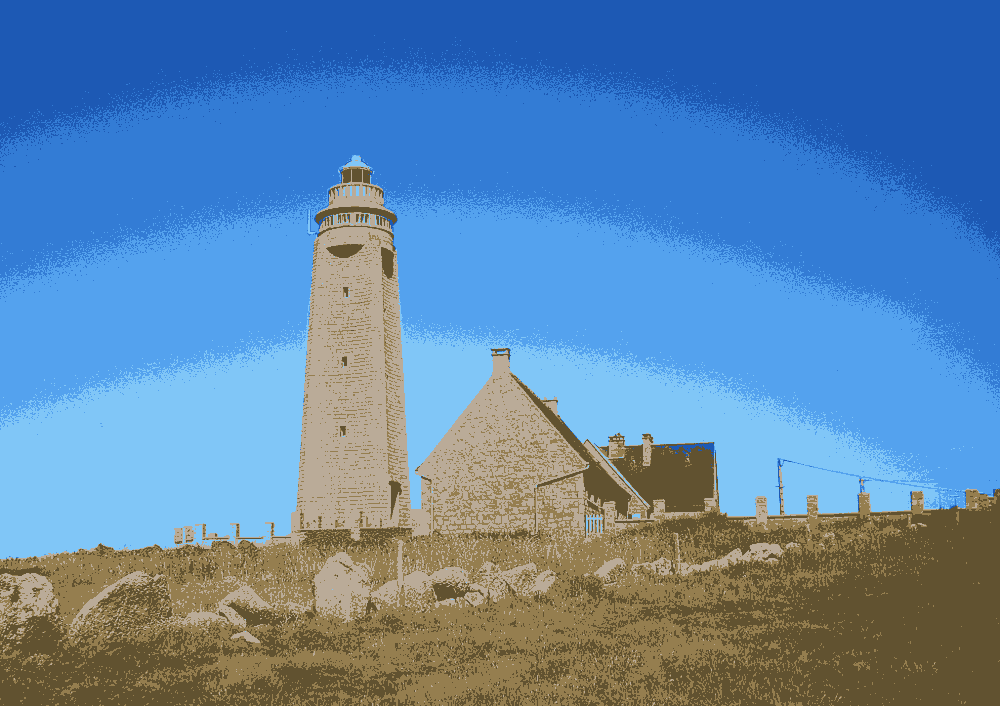
\includegraphics[width=6cm]{./imgkmeanscluster01-07.png}\\
\centering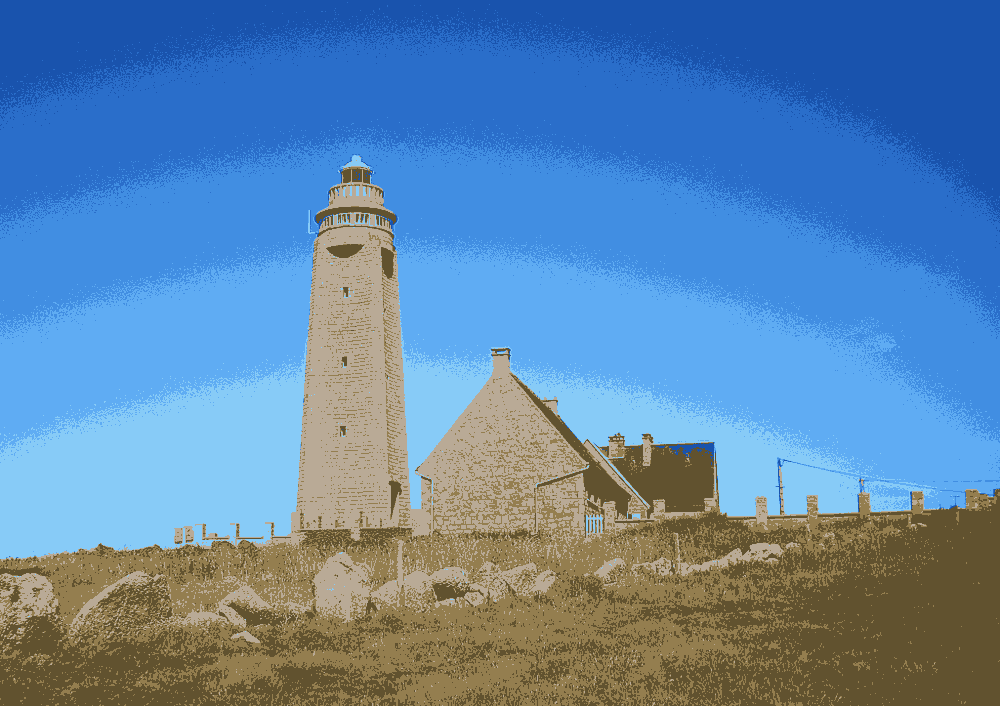
\includegraphics[width=6cm]{./imgkmeanscluster01-08.png}
\centering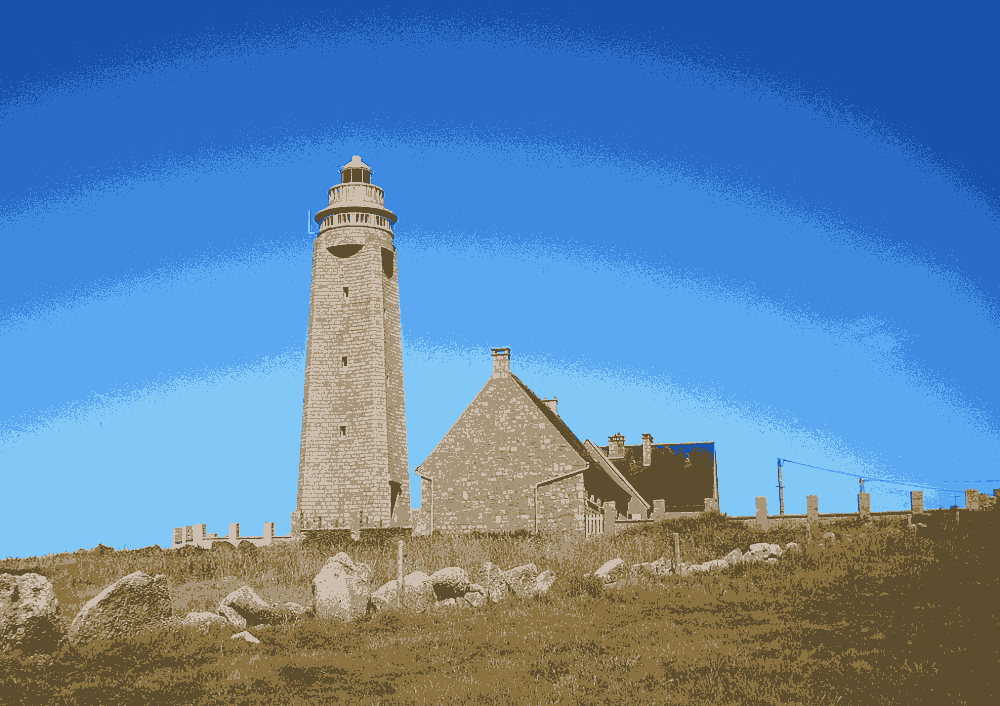
\includegraphics[width=6cm]{./imgkmeanscluster01-09.png}\\
\centering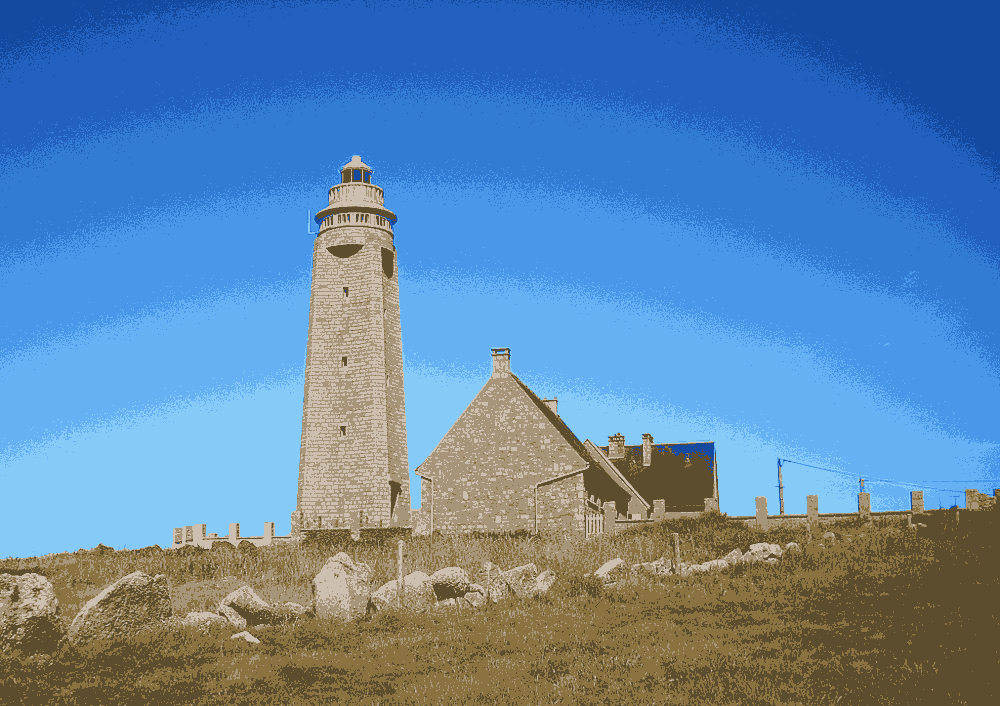
\includegraphics[width=6cm]{./imgkmeanscluster01-10.png}\\
\end{figure}
\end{center}

imgkmeanscluster02.tga:\\
\begin{center}
\begin{figure}[H]
\centering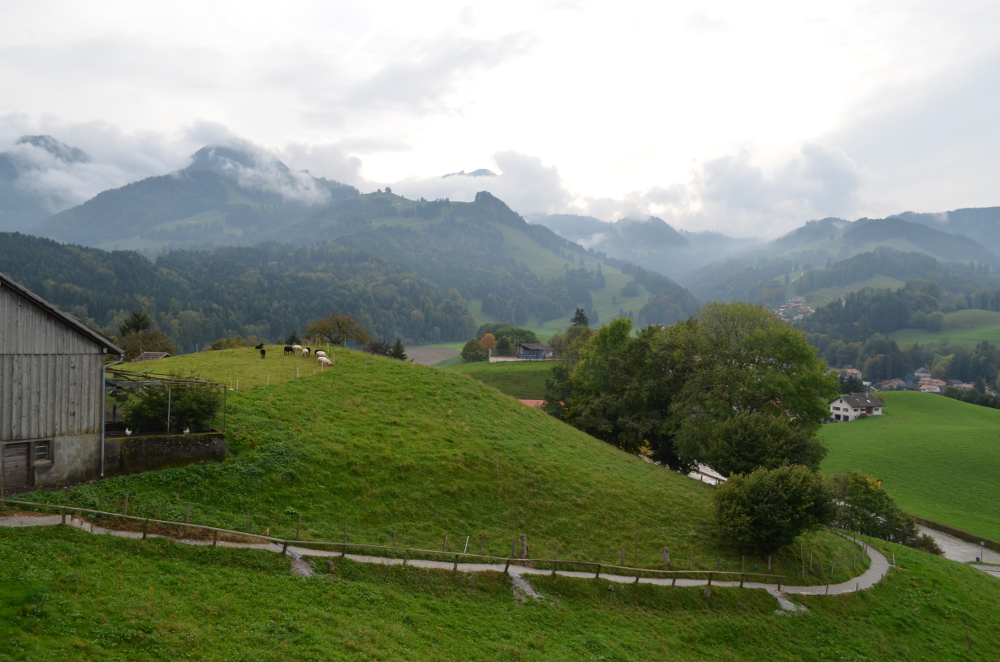
\includegraphics[width=6cm]{./imgkmeanscluster02.png}\\
\end{figure}
\end{center}

clustering for K equals 2 to 10:\\
\begin{center}
\begin{figure}[H]
\centering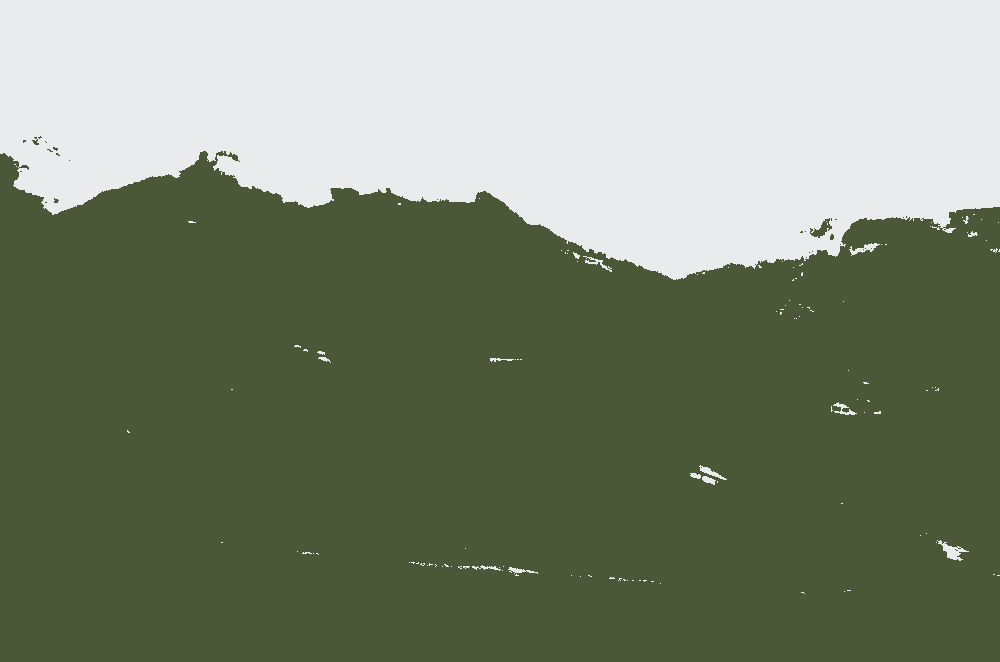
\includegraphics[width=6cm]{./imgkmeanscluster02-02.png}
\centering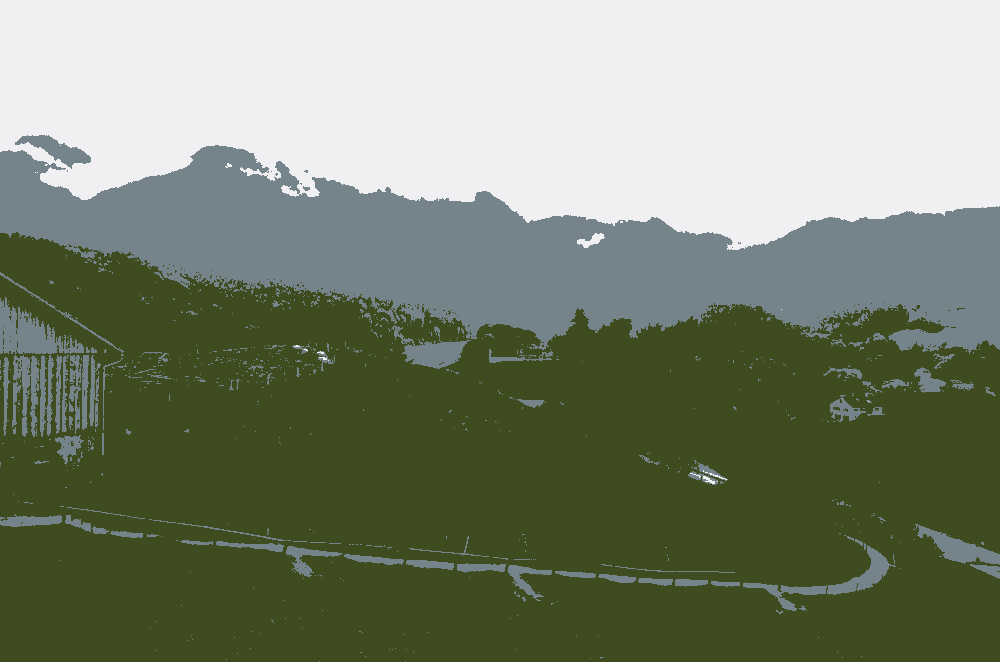
\includegraphics[width=6cm]{./imgkmeanscluster02-03.png}\\
\centering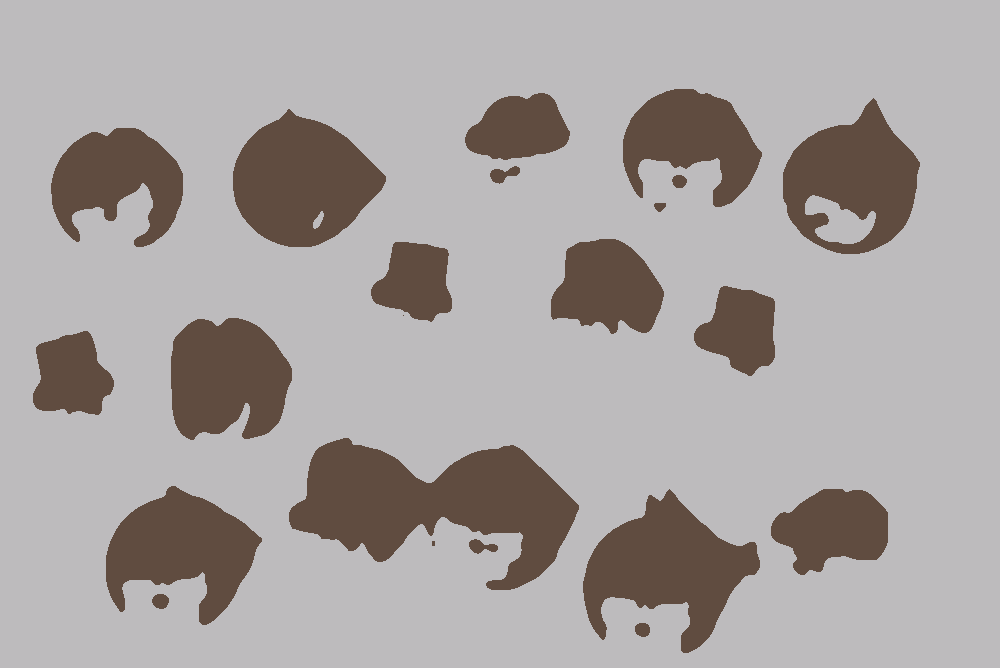
\includegraphics[width=6cm]{./imgkmeanscluster02-04.png}
\centering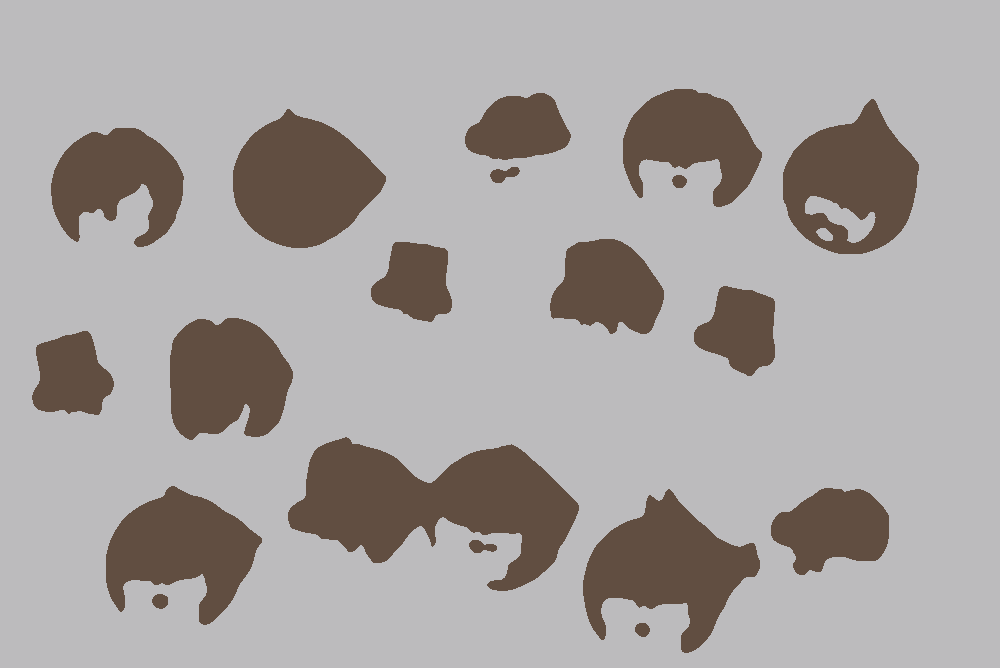
\includegraphics[width=6cm]{./imgkmeanscluster02-05.png}\\
\centering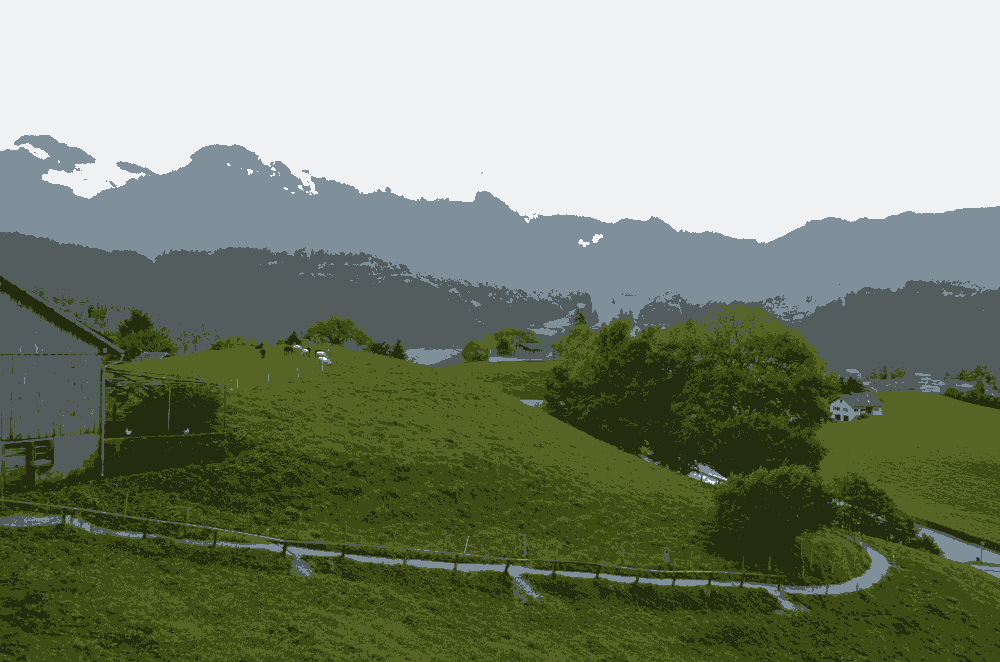
\includegraphics[width=6cm]{./imgkmeanscluster02-06.png}
\centering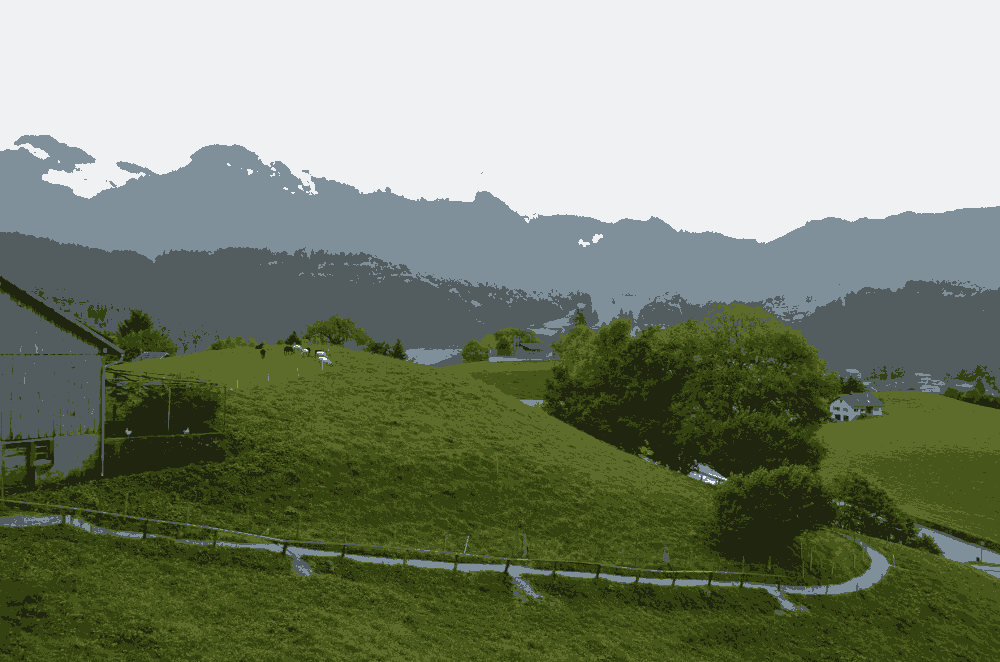
\includegraphics[width=6cm]{./imgkmeanscluster02-07.png}\\
\centering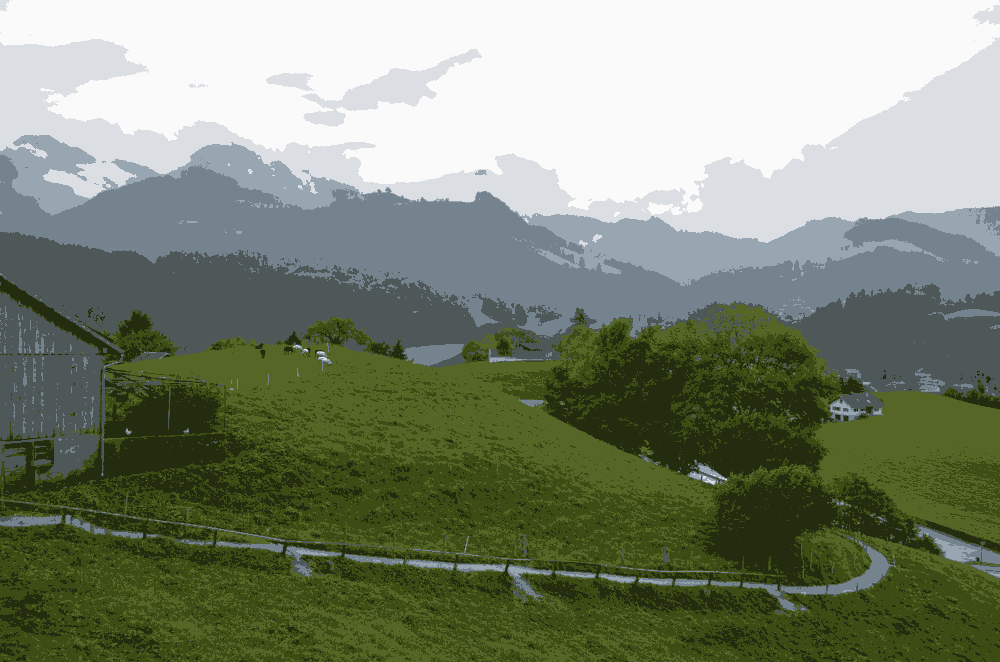
\includegraphics[width=6cm]{./imgkmeanscluster02-08.png}
\centering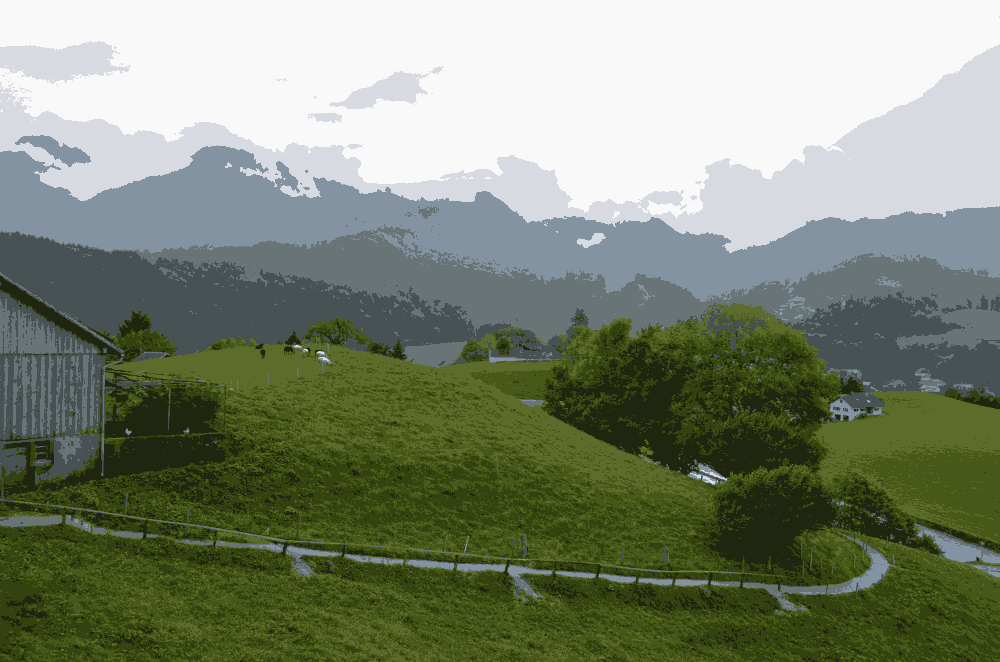
\includegraphics[width=6cm]{./imgkmeanscluster02-09.png}\\
\centering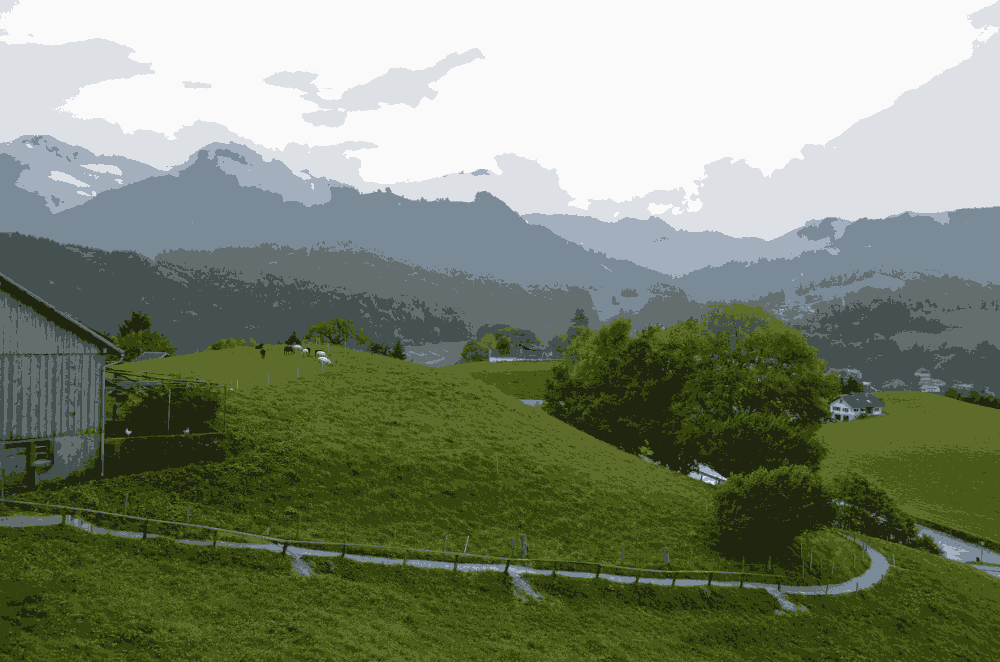
\includegraphics[width=6cm]{./imgkmeanscluster02-10.png}
\end{figure}
\end{center}
